
\documentclass[nooutcomes]{ximera}
%\documentclass[space,handout,nooutcomes]{ximera}

% For preamble materials

\usepackage{pgf,tikz}
\usepackage{mathrsfs}
\usetikzlibrary{arrows}
\usepackage{framed}
\usepackage{amsmath}
%\pgfplotsset{compat=1.16}

\graphicspath{
  {./}
  {algorithms/}
  {../algorithms/}
}

\pdfOnly{\renewenvironment{image}[1][]{\begin{center}}{\end{center}}}

%%% This set of code is all of our user defined commands
\newcommand{\bysame}{\mbox{\rule{3em}{.4pt}}\,}
\newcommand{\N}{\mathbb N}
\newcommand{\C}{\mathbb C}
\newcommand{\W}{\mathbb W}
\newcommand{\Z}{\mathbb Z}
\newcommand{\Q}{\mathbb Q}
\newcommand{\R}{\mathbb R}
\newcommand{\A}{\mathbb A}
\newcommand{\D}{\mathcal D}
\newcommand{\F}{\mathcal F}
\newcommand{\ph}{\varphi}
\newcommand{\ep}{\varepsilon}
\newcommand{\aph}{\alpha}
\newcommand{\QM}{\begin{center}{\huge\textbf{?}}\end{center}}

\renewcommand{\le}{\leqslant}
\renewcommand{\ge}{\geqslant}
\renewcommand{\a}{\wedge}
\renewcommand{\v}{\vee}
\renewcommand{\l}{\ell}
\newcommand{\mat}{\mathsf}
\renewcommand{\vec}{\mathbf}
\renewcommand{\subset}{\subseteq}
\renewcommand{\supset}{\supseteq}
\renewcommand{\emptyset}{\varnothing}
\newcommand{\xto}{\xrightarrow}
\renewcommand{\qedsymbol}{$\blacksquare$}
\newcommand{\bibname}{References and Further Reading}
\renewcommand{\bar}{\protect\overline}
\renewcommand{\hat}{\protect\widehat}
\renewcommand{\tilde}{\widetilde}
\newcommand{\tri}{\triangle}
\newcommand{\minipad}{\vspace{1ex}}
\newcommand{\leftexp}[2]{{\vphantom{#2}}^{#1}{#2}}

%% More user defined commands
\renewcommand{\epsilon}{\varepsilon}
\renewcommand{\theta}{\vartheta} %% only for kmath
\renewcommand{\l}{\ell}
\renewcommand{\d}{\, d}
\newcommand{\ddx}{\frac{d}{dx}}
\newcommand{\dydx}{\frac{dy}{dx}}


\usepackage{bigstrut}


\newenvironment{sectionOutcomes}{}{}

\usepackage{array}
%\setlength{\extrarowheight}{-.2cm}   % Commented out by Findell to fix table headings.  Was this for typesetting division?  
\newdimen\digitwidth
\settowidth\digitwidth{9}
\def~{\hspace{\digitwidth}}
\def\divrule#1#2{
\noalign{\moveright#1\digitwidth
\vbox{\hrule width#2\digitwidth}}}


\title{Fractions}
\author{Bart Snapp and Brad Findell and Jenny Sheldon}
\begin{document}
\begin{abstract}
Problems about rational numbers.
\end{abstract}
\maketitle


%\begin{problem}
%Problem
%\begin{freeResponse}
%\begin{hint}
%Hint
%\end{hint}
%\end{freeResponse}
%\end{problem} 


\begin{problem}
Select all numbers below which are fractions.
\begin{selectAll}
	\choice[correct]{$\frac{4}{9}$}
	\choice{$0$}
	\choice{$e$}
	\choice[correct]{$\frac{\sqrt{3}}{12}$}
	\choice[correct]{$\frac{-\pi}{3}$}
	\choice[correct]{$\frac{-23}{387}$}
	\choice{$-2.9734$}
\end{selectAll}
\end{problem}



\begin{problem}
Select all numbers below which are rational numbers.
\begin{selectAll}
	\choice[correct]{$\frac{4}{9}$}
	\choice[correct]{$0$}
	\choice{$e$}
	\choice{$\frac{\sqrt{3}}{12}$}
	\choice{$\frac{-\pi}{3}$}
	\choice[correct]{$\frac{-23}{387}$}
	\choice[correct]{$-2.9734$}
\end{selectAll}
\end{problem}



\begin{problem}
Here's a tricky one!  True or false: $\frac{\sqrt{2}}{\sqrt{8}}$ is a rational number.
\begin{hint}
	Can you simplify this number at all?
\end{hint}
\begin{multipleChoice}
\choice[correct]{True}
\choice{False}
\end{multipleChoice}
\end{problem}




\begin{problem}
Ashleigh has a brownie recipe that calls for $\frac{2}{9}$ of a tablespoon of baking powder.  (She has some crazy measuring cups at home!). To represent her tablespoon of baking powder, she draws the following rectangle.
\begin{center} 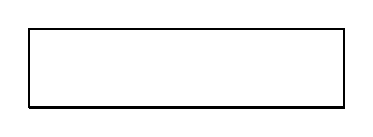
\begin{tikzpicture}
	\draw[thick] (0,0)--(4,0)--(4,1)--(0,1)--(0,0);
\end{tikzpicture} \end{center}

To represent her $\frac{2}{9}$ of a tablespoon, into how many equal-sized pieces should she cut the entire rectangle?  Give the most basic answer you can.

\begin{prompt}
She should cut the rectangle into $ \answer[given]{9}$ equal-sized pieces.
\end{prompt}

To represent her $\frac{2}{9}$ of a tablespoon, how many of those pieces should she shade?  Give the most basic answer you can.

\begin{prompt}
She should shade $\answer[given]{2}$ pieces.
\end{prompt}

\end{problem}



\begin{problem}
In the previous problem, the question asked for ``the most basic answer'' that you could give.  Why was the question phrased in that way?  What other kinds of answers might there be?
\begin{freeResponse}
\begin{hint}
	There are infinitely many fractions which are equivalent to $\frac{2}{9}$.  If we were not looking for the most basic answer, we might cut our whole into $27$ pieces, and shade $6$ of them.  Or, we might cut our whole into $90$ pieces, and shade $20$ of those pieces.
\end{hint}
\end{freeResponse}
\end{problem}




\begin{problem}
The image below depicts a fraction whose whole is the entire rectangle.  What fraction of the entire rectangle is shaded?
\begin{center} 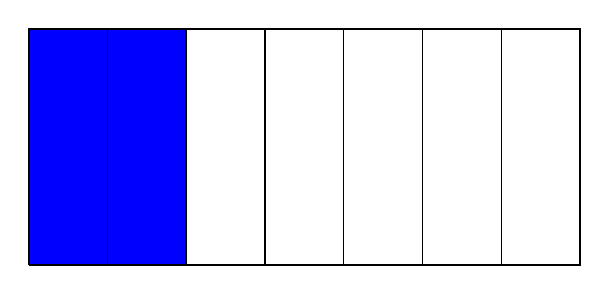
\begin{tikzpicture}
	\draw[thick, fill=blue]  (0,0) -- (2,0) -- (2,3) -- (0,3)--(0,0);
	\draw[thick] (0,0) -- (7,0) -- (7,3) -- (0,3)--(0,0);
	\foreach \x in {1,2,3,4,5,6} \draw (\x,0)--(\x,3);
\end{tikzpicture}\end{center}

\begin{prompt}
We see that $\frac{\answer[given]{2}}{\answer[given]{7}}$ of the rectangle is shaded.
\end{prompt}

\end{problem}



\begin{problem}
The image below depicts a fraction whose whole is the blue shaded region.  What fraction is the entire drawing of the blue shaded region?
\begin{center} 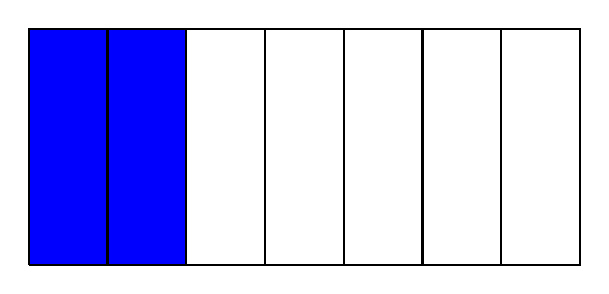
\begin{tikzpicture}
	\draw[thick, fill=blue]  (0,0) -- (2,0) -- (2,3) -- (0,3)--(0,0);
	\draw[thick] (0,0) -- (7,0) -- (7,3) -- (0,3)--(0,0);
	\foreach \x in {1,2,3,4,5,6} \draw[thick] (\x,0)--(\x,3);
\end{tikzpicture}\end{center}

\begin{prompt}
We see that the rectangle is $\frac{\answer[given]{7}}{\answer[given]{2}}$ of the shaded region.
\end{prompt}

\end{problem}




\begin{problem}
The image below depicts a fraction whose whole is the entire rectangle.  What fraction of the entire rectangle is shaded?
\begin{center} 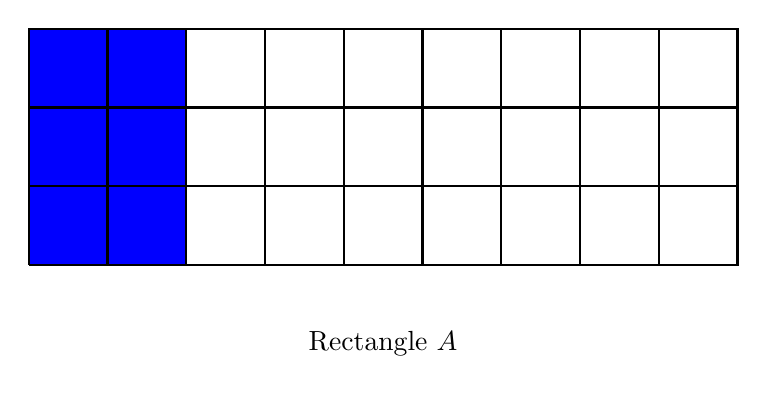
\begin{tikzpicture}
	\draw[thick, fill=blue]  (0,0) -- (2,0) -- (2,3) -- (0,3)--(0,0);
	\draw[thick] (0,0) -- (9,0) -- (9,3) -- (0,3)--(0,0);
	\foreach \x in {1,2,3,4,5,6,7,8} \draw[thick] (\x,0)--(\x,3);
	\foreach \y in {1,2} \draw[thick] (0,\y)--(9,\y);
	\node at (4.5, -1) {Rectangle $A$};
\end{tikzpicture}\end{center}

\begin{prompt}
We see that $\frac{\answer[given]{6}}{\answer[given]{27}}$ of the rectangle is shaded.
\end{prompt}

\begin{problem}
Compare the rectangle above (Rectangle $A$) with the one below (Rectangle $B$).  
\begin{center} 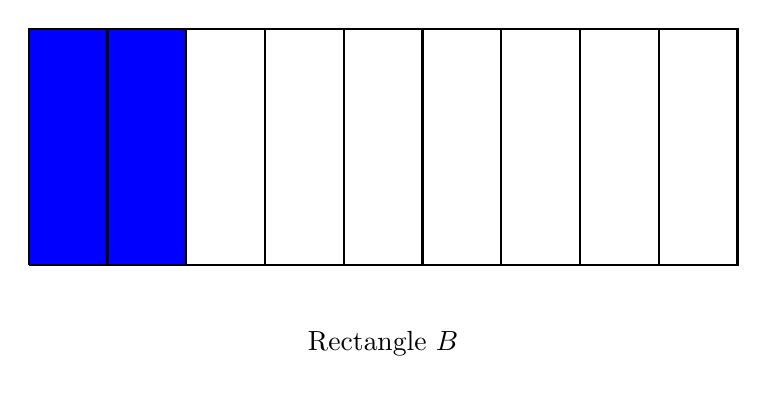
\begin{tikzpicture}
	\draw[thick, fill=blue]  (0,0) -- (2,0) -- (2,3) -- (0,3)--(0,0);
	\draw[thick] (0,0) -- (9,0) -- (9,3) -- (0,3)--(0,0);
	\foreach \x in {1,2,3,4,5,6,7,8} \draw[thick] (\x,0)--(\x,3);
	\node at (4.5, -1) {Rectangle $B$};
\end{tikzpicture}\end{center}

How could we have obtained Rectangle $A$'s drawing from the drawing of Rectangle $B$?  Choose the best answer below.
\begin{multipleChoice}
\choice{The pictures are unrelated.}
\choice{We multiplied the picture by $3$.}
\choice[correct]{We split each of the pieces in the whole for Rectangle $B$ into three equal pieces.}
\choice{We drew two more horizontal lines on the picture.}
\end{multipleChoice}


\begin{problem}
 Comparing Rectangle $A$ and Rectangle $B$, we can see the equivalence of which two fractions?
 
 \begin{prompt}
 We see that $\frac{\answer[given]{2}}{9}$ is equivalent to $\frac{\answer[given]{6}}{27}$.
 \end{prompt}
 
 \begin{problem}
 Explain exactly how we can see from the two diagrams that the fractions are equivalent.
 \begin{freeResponse}
 \begin{hint}
 First, notice that we start with the same whole in each picture.  When we cut each of the nine pieces of Rectangle $B$ into three pieces, we end up with $27$ pieces making up our whole.  At the same time (without doing any more work!) we have also managed to cut each of the original two shaded pieces into three pieces each, leaving us with $6$ shaded pieces.  The shading didn't change at all, and the total amount didn't change at all, so the quantities represented by the two fractions have to be the same.
 \end{hint}
 \end{freeResponse}
 
 
\end{problem}
\end{problem}
\end{problem}
\end{problem}


\begin{problem}
What fraction of the entire rectangle is shaded?

\begin{center} 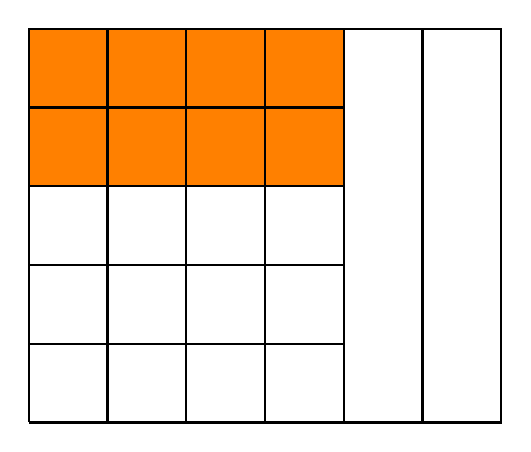
\begin{tikzpicture}
	\draw[fill=orange] (0,5)--(0,3)--(4,3)--(4,5)--(0,5);
	\draw[thick] (0,0)--(6,0)--(6,5)--(0,5)--(0,0);
	\foreach \x in {1, 2, 3, 4,5} \draw[thick] (\x, 0)--(\x,5);
	\foreach \y in {1, 2, 3, 4} \draw[thick] (0, \y)--(4, \y);
\end{tikzpicture}\end{center}

\begin{prompt}
We see that $\answer[given]{\frac{8}{30}}$ of the rectangle is shaded.
\end{prompt}

\begin{problem}
	Let's think of the orange shaded area as the result of multiplying two fractions. What are these fractions?
	
	\begin{prompt}
	If we imagine extending the horizontal lines all the way across our rectangle, we can view one whole group as containing $\answer[given]{\frac{2}{5}}$ of the entire rectangle.  (This would be the continuation of the orange region horizontally across the rectangle.) Then, we can see that we have shaded $\answer[given]{\frac{4}{6}}$ of that group.  Thus, our multiplication problem would be $\answer[given]{\frac{4}{6}} \times \answer[given]{\frac{2}{5}}$.
	
	\begin{hint}
	Remember: for our meaning of multiplication, the order of the factors matters!
	\end{hint}
	\end{prompt}
\end{problem}

\end{problem}





\end{document}



